%-------------------------------------------------------------------------------
\section{Scalability}
\label{sec:scalability}
%-------------------------------------------------------------------------------

While \cref{sec:results} presents results for {\em current} BGP tables, this section presents scalability analysis for \resail and \bsic on larger {\em synthetic} routing databases. We omit scalability analysis for \mashup because it requires too much TCAM (for Tofino-2).

\subsection{IPv4 Scaling} \label{subsec:ipv4_scaling}

\begin{figure}
\centering
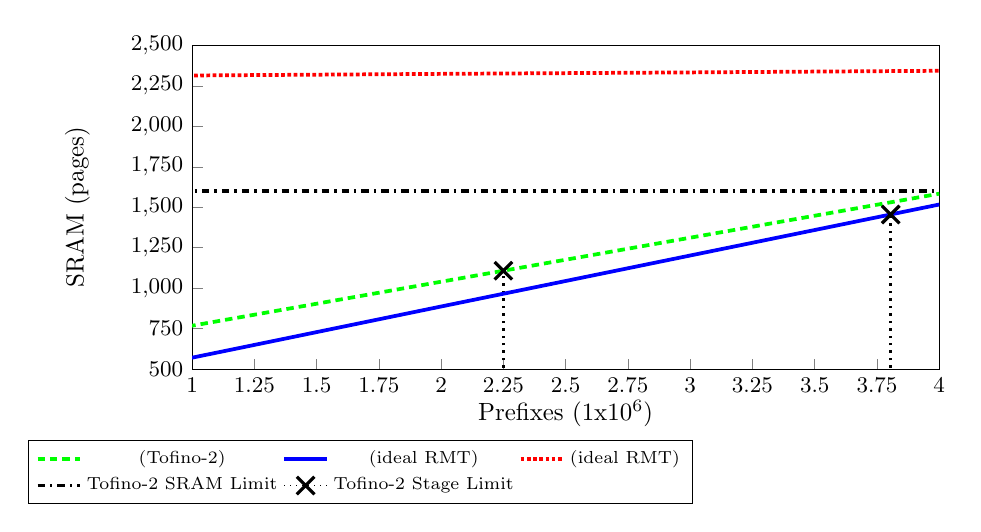
\begin{tikzpicture}[scale=0.9]
    \normalsize
    \begin{axis}[
        xlabel=Prefixes (1x$10^6$),
        ylabel=SRAM (pages),
        xmin=1, xmax=4,
        ymin=500, ymax=2500,
        xtick={1,1.25,...,4},
        ytick={500,750,...,2500},
        width=\columnwidth,
        height=175pt,
        xticklabel style={rotate=0,font=\small},
        yticklabel style={rotate=0,font=\small},
        xlabel style={font=\normalsize,at={(axis description cs:.5,-.07)}},
        ylabel style={font=\normalsize,at={(axis description cs:-.125,.5)}},
        legend columns=3,
        legend style={at={(-0.22,-0.22)},anchor=north west,font=\scriptsize},
        tick pos=left
    ]
    
    \draw[dotted, black, line width=1pt] plot[domain=0:4] (3.805000, 0) -- (3.805000, 1455);
    \draw[dotted, black, line width=1pt] plot[domain=0:4] (2.250000, 0) -- (2.250000, 1108);

    \addplot[line width=1.5pt,mark=none,densely dashed,color=green,domain=0:4] {271.8*x + 496.5};
    \addlegendentry{\resail (Tofino-2)}
    
    \addplot[line width=1.5pt,mark=none,smooth,color=blue]
    plot coordinates {
        (0.932861,556)
        (1.000000,571)
        (2.000000,887)
        (3.000000,1202)
        (3.800000,1454)
        (4.000000,1517)
    };
    \addlegendentry{\resail (ideal RMT)}
    \addplot[line width=1.5pt,mark=none,densely dotted,color=red]
    plot coordinates {
        (0.932861,2313)
        (1.000000,2314)
        (2.000000,2324)
        (3.000000,2333)
        (3.800000,2341)
        (4.000000,2343)
    };
    \addlegendentry{\sail (ideal RMT)}

    \addplot[line width=1.5pt,mark=none,dash pattern=on 3pt off 2pt on 1pt off 2pt,color=black,domain=0:4] {1600};
    \addlegendentry{Tofino-2 SRAM Limit}

    \addplot[dotted,mark=x,mark size=5pt,mark options={solid, line width=1.3pt}] coordinates {(2.250000, 1108)};
    \addplot[dotted,mark=x,mark size=5pt,mark options={solid, line width=1.3pt}] coordinates {(3.805000, 1455)}; 
    \addlegendentry{Tofino-2 Stage Limit}
    
    \end{axis}
\end{tikzpicture}
\caption{\resail vs \sail scaling (IPv4)}
\label{fig:ipv4_scaling}
\vspace{-\baselineskip}
\end{figure}

\cref{fig:ipv4_scaling} shows IPv4 scalability results for \resail and our SRAM-only IPv4 baseline, \sail. We did not generate synthetic prefixes because the resource utilization of \resail and \sail depends on the distribution of {\em prefix lengths} rather than the distribution of the prefixes themselves. From the perspective of memory usage, \resail and \sail do not distinguish between prefixes of identical length. Therefore, we use a simple scaling model that applies a constant scaling factor to all prefix lengths. For the ideal RMT results of \resail and \sail, we use the steps described in \cref{subsec:target_implementations} to calculate their new utilization. For the Tofino-2 results of \resail, we update the corresponding P4 table sizes to reflect the larger databases.

For ideal RMT, \sail is infeasible because its SRAM cost far exceeds the Tofino-2 SRAM limit. At any given database size, \resail for Tofino-2 uses more SRAM than \resail for ideal RMT. This is expected since Tofino-2 does not allow 100\% SRAM utilization. Notably, \resail on an ideal RMT chip scales to around 3.8 million prefixes, 4X larger than the current IPv4 BGP table. \resail on Tofino-2 scales to around 2.25 million prefixes, 2.3X larger than the current routing database and significantly beyond \sail's capacity.

\subsection{IPv6 Scaling} \label{subsec:ipv6_scaling}

\begin{figure}
\centering
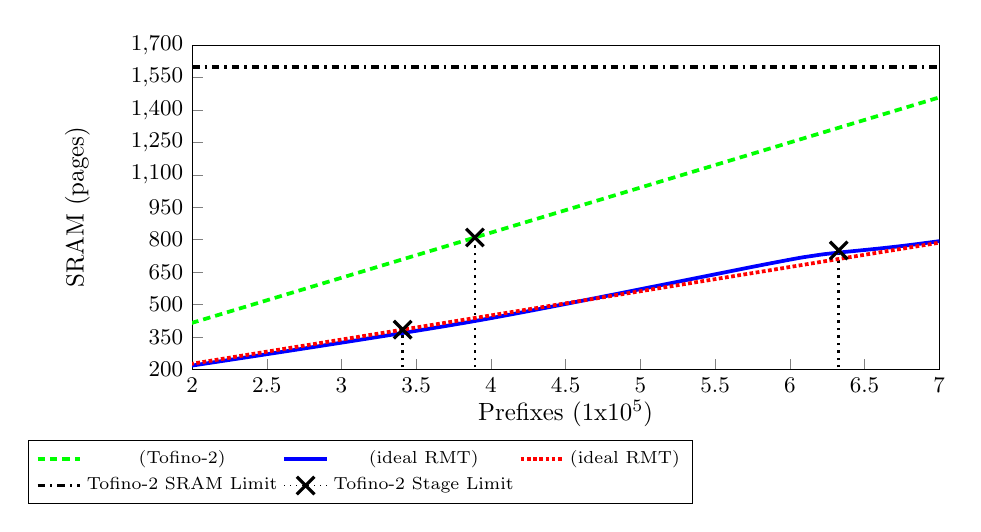
\begin{tikzpicture}[scale=0.9]
    \normalsize
    \begin{axis}[
        xlabel=Prefixes (1x$10^5$),
        ylabel=SRAM (pages),
        xmin=2, xmax=7,
        ymin=200, ymax=1700,
        xtick={2,2.5,...,7},
        ytick={200,350,...,1700},
        width=\columnwidth,
        height=175pt,
        xticklabel style={rotate=0,font=\small},
        yticklabel style={rotate=0,font=\small},
        xlabel style={font=\normalsize,at={(axis description cs:.5,-.07)}},
        ylabel style={font=\normalsize,at={(axis description cs:-.125,.5)}},
        legend columns=3,
        legend style={at={(-0.22,-0.22)},anchor=north west,font=\scriptsize},
        tick pos=left
    ]
    
    \draw[dotted, black, line width=1pt] plot[domain=0:7] (6.32717, 0) -- (6.32717, 750);
    \draw[dotted, black, line width=1pt] plot[domain=0:7] (3.89269, 0) -- (3.89269, 810);
    \draw[dotted, black, line width=1pt] plot[domain=0:7] (3.40943, 0) -- (3.40943, 383);

    \addplot[line width=1.5pt,mark=none,densely dashed,color=green,domain=0:7] {208.9*x - 3.335};
    \addlegendentry{\bsic (Tofino-2)}
    
    \addplot[line width=1.5pt,mark=none,smooth,color=blue]
    plot coordinates {
        (1.94635,211)
        (3.89269,423)
        (5.83903,686)
        (6.16385,726)
        (6.32717,740)
        (6.81401,776)
        (7.78537,867)
    };
    \addlegendentry{\bsic (ideal RMT)}
    \addplot[line width=1.5pt,mark=none,densely dotted,color=red]
    plot coordinates {
        (1.94635,219)
        (3.89270,437)
        (5.83905,655)
        (6.36743,715)
        (7.13538,801)
    };
    \addlegendentry{\hibst (ideal RMT)}

    \addplot[line width=1.5pt,mark=none,dash pattern=on 3pt off 2pt on 1pt off 2pt,color=black,domain=0:7] {1600};
    \addlegendentry{Tofino-2 SRAM Limit}

    \addplot[dotted,mark=x,mark size=5pt,mark options={solid, line width=1.3pt}] coordinates {(6.32717, 750)};
    \addplot[dotted,mark=x,mark size=5pt,mark options={solid, line width=1.3pt}] coordinates {(3.89269, 810)};
    \addplot[dotted,mark=x,mark size=5pt,mark options={solid, line width=1.3pt}] coordinates {(3.40943, 383)};
    \addlegendentry{Tofino-2 Stage Limit}
    
    \end{axis}
\end{tikzpicture}
\caption{\bsic vs \hibst scaling (IPv6)}
\label{fig:ipv6_scaling}
\vspace{-\baselineskip}
\end{figure}

\cref{fig:ipv6_scaling} shows IPv6 scalability results for \bsic and our SRAM-only IPv6 baseline, \hibst. For \bsic, we generated synthetic prefixes because its resource utilization depends on the distribution of prefixes and sub-prefixes. To obtain worst-case scalability results, observe that the first three bits of IPv6 prefixes in AS131072 are 000---forming an {\em IPv6 universe}. We use different combinations of these bits to generate significantly larger synthetic databases from AS131072, an approach we call {\em multiverse scaling}. Multiverse scaling assumes that the distribution of all prefix lengths scales uniformly. In practice, customer scaling causes some prefixes (e.g., /48s) to scale more rapidly than others (e.g., /24s). However, this stresses only the BSTs and not the initial TCAM, unlike multiverse scaling which models worst-case results for TCAM, SRAM, and stages. For \hibst, we use the memory calculation provided in \cite{hibst}.

As seen in \cref{fig:ipv6_scaling}, both instances of \bsic are able to out-scale \hibst. For an ideal RMT chip, \hibst only scales to around 340k prefixes, 1.8X larger than the current IPv6 BGP Table. Even though \hibst is the most memory efficient IPv6 lookup scheme, it requires too many stages. Comparing the two instances of \bsic, we see that \bsic for ideal RMT scales to around 630k prefixes, 3.3X larger than the current routing database. Since \bsic for Tofino-2 uses over 2X more stages, it scales to around 390k prefixes---2X the size of the current IPv6 BGP table.